\chapter{Delimitations}

Due to constrain of our time during this project, designing a new demining robot product that could satisfy the optimal requirements are unattainable. Thus we will be working on a prototype robot for this project, the turtlebot 2 will be used and more specifically the Kobuki platform which is an prototype base, due to the fact that it can be used for prototyping regarding the main part of our requirements. The main idea is that the prototype code would be implemented on a full-scale demining robot, with the correct sensors, wheels and locomotion. The kobuki base still has a lot of these attributes, which can be tested or delimited in a prototype environment. 

\vspace{2mm}

These limitations included not being able to move in various terrain, and it is not at all functional regarding locating a large spectrum of mine types. The turtlebot has differential drive locomotion which is alright for the steering, but the wheels does not have great traction in a rocky or sandy terrain like Afghanistan - due to it's small wheels, thus it is hard to test these aspects in a rough terrain and therefore the project group will be delimiting the requirements to fit an indoor environment instead of the robots \"natural habitat\".

\begin{figure}[h]
    \centering
        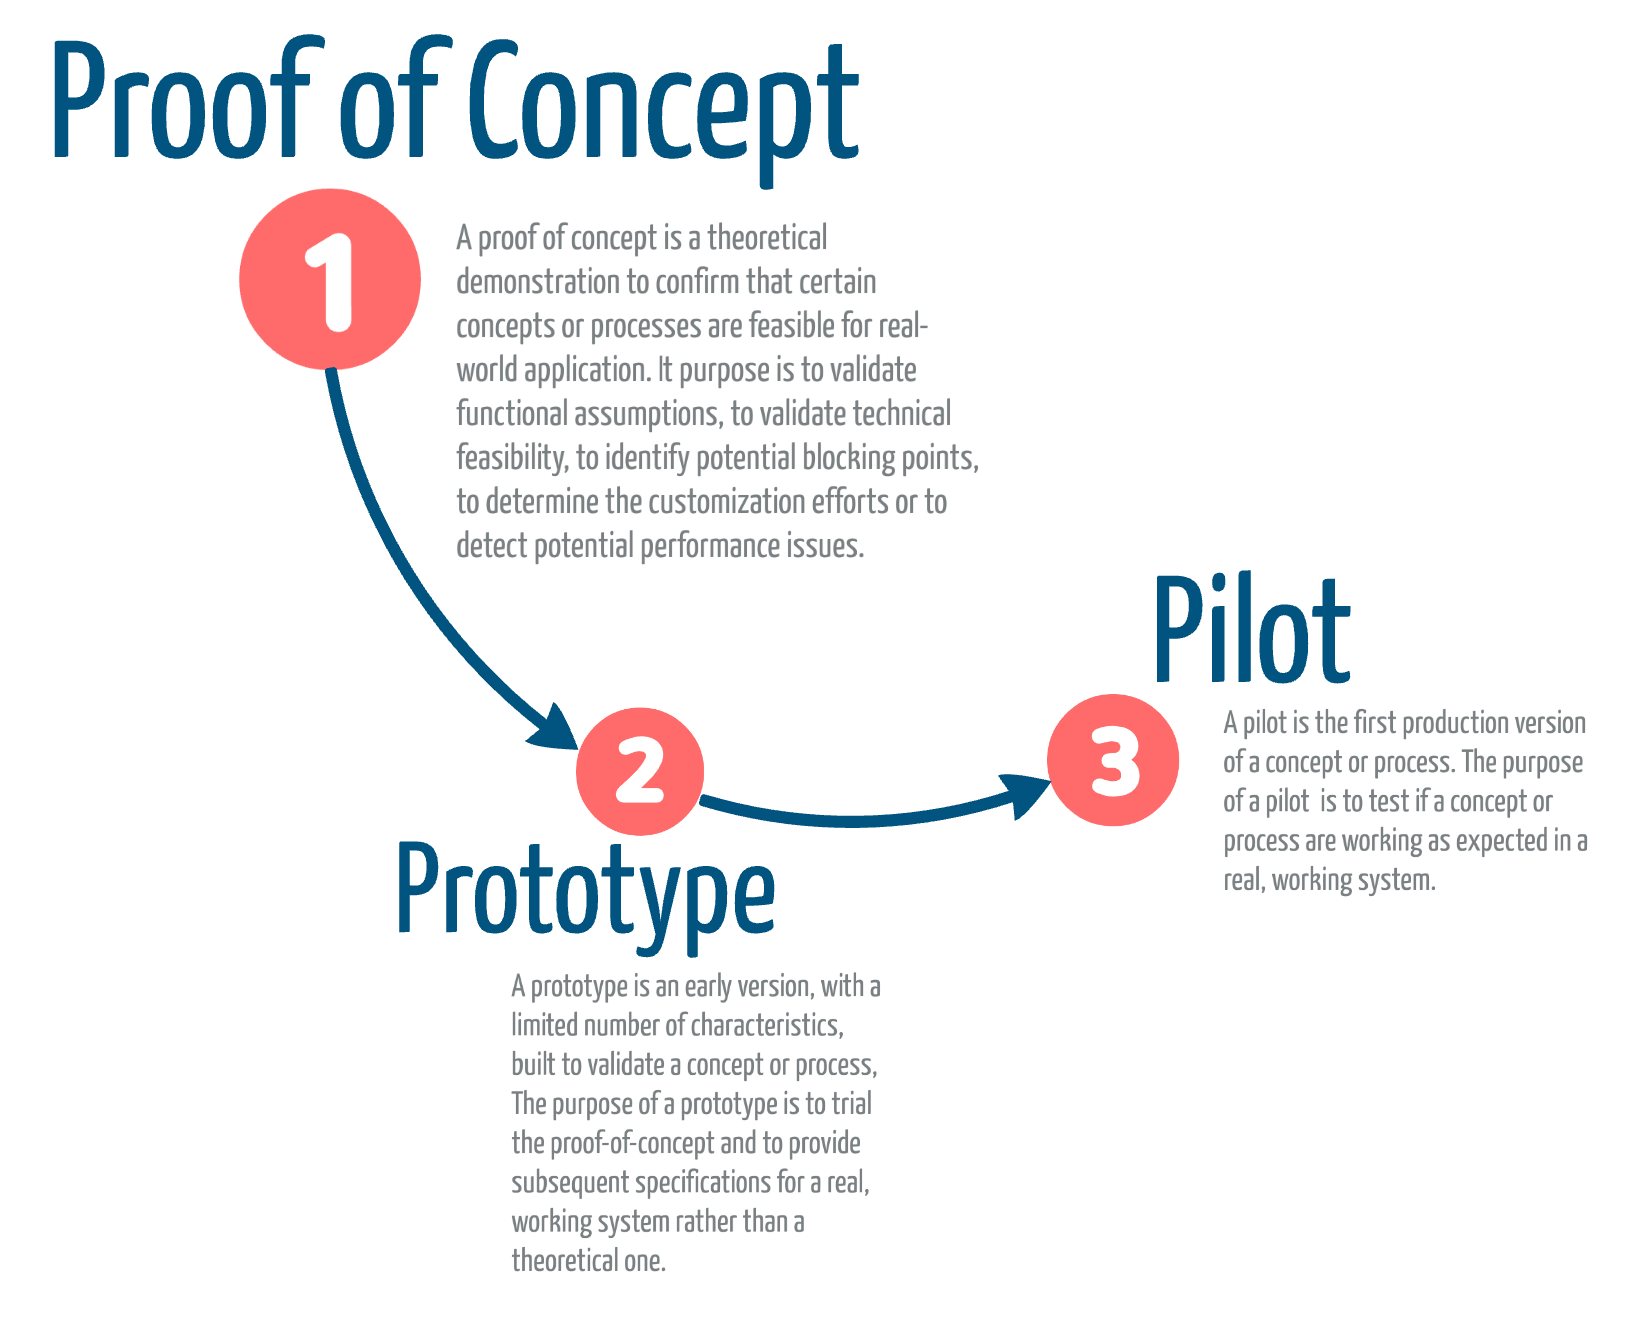
\includegraphics[width=12cm]{00 - Images/POC-reusable-license.PNG}
    \caption{Proof of concept diagram - Daniel Velasco: Under reusable license}
    \label{fig:POC}
  \end{figure}

\section{A Delimited Problem Statement}\label{delimit_statement}
How can we make the Turtlebot 2, act as proof of concept for the part of our final problem statement which addresses the need for an algorithm to make a robot map an area while in the process of locating objects with our modified proof of concept metalsensor, which have the same attributes as various landmines

  \newpage

  \newgeometry{left=0.2cm,right=0.2cm}
  \begin{center}
  \begin{longtable}{| c | L{4.5cm} | L{9cm} | L{4.5cm} |}
  \caption{Prototype requirements} \label{tab:long2 } \\
  \hline 
  \multicolumn{1}{|c|}{\textbf{\#}} 
  & \multicolumn{1}{c|}{\textbf{Name}} 
  & \multicolumn{1}{c|}{\textbf{Description}} 
  & \multicolumn{1}{c|}{\textbf{Testing}}\\ 
  \hline 
  \endfirsthead
  
  \multicolumn{3}{c}%
  {{\bfseries \tablename\ \thetable{} -- continued from previous page}} \\
  \hline
  \multicolumn{1}{|c|}{\textbf{\#}} 
  & \multicolumn{1}{c|}{\textbf{Name}} 
  & \multicolumn{1}{c|}{\textbf{Description}} 
  & \multicolumn{1}{c|}{\textbf{Testing}}\\ 
  \hline 
  \endhead
  
  \hline \multicolumn{4}{|r|}{{Continued on next page}} \\ \hline
  \endfoot
  
  \hline \hline
  \endlastfoot
  
  1\label{req8.1-p} 
  & Start/stop
  & The robot should perform primary objectives autonomously, but report to an operator when errors occur, at any point the operator should be able to start, stop and take manual control of the operation.
  & Section \ref{T1}
  \\
  \hline
  2
  & Mapping 
  & The robot should be able to map the surrounding environment to a .pgm image file with corresponding .yaml definition file.
  & Section \ref{T2}
  \\
  \hline
  3 
  & Map Structure 
  & The robot should be able to divide a given environment map into a grid with a width of 350mm, for the purpose of plotting a search route.
  & Section \ref{T3}
  \\
  \hline
  4 & Navigation 
  & The robot should be able to navigate autonomously \st{through a variety of terrains in Afghanistan}\footnote{Delimitation: At this point it is not possible to test the prototype robot in various terrain of Afhghanistan.\\}, using the .yaml environment map.
  & Section \ref{T4}
  \\ 
  \hline 
  5 
  & Edge Detection
  & The robot should be able to detect shifts in the terrain to avoid falling down a steep hill or down a cliff.
  & Section \ref{T5}
  \\
  \hline
  6
  & Obstacle Avoidance
  & The robot should be able to detect obstacles in its current path, thus interrupt the current path and calculate a new path, furthermore the robot should avoid previous located mines \label{req.4-p}.
  & Section \ref{T6}
  \\
  \hline
  ND 
  & Mine Triggering 
  & \st{The robot should not exceed a weight of $\sim$6kg to ensure that it does not trigger landmines when approximating these.}\footnote{Ruled out:, At this point it is not possible to test the final weight - Due to the fact, that it is not the final robot.}
  & Ruled out
  \\
  \hline
  7 
  & Mine Detection 
  & The robot should be able to detect \st{mines} objects made of metal \st{and/or other materials such as plastic or glass} - in \st{or above the ground}\footnote{Delimitation: The prototype robot will not be able to find mines made of metal, plastic or glass. It is only mounted with a prototype metal detector, which can detect metal objects on the ground to act as a proof of concept.\\}, furthermore it should be able to approximate which type of mine it has located.
  & Section \ref{T7}
  \\
  \hline
  8
  & Mine Flagging 
  & The robot should be able to flag a found mine (with respect to table \ref{req8.1-p} - \#5), both in a virtual map and with a physical interaction eg. Spray paint \textit{(Red: \gls{ap}, Blue: \gls{at})}.
  & Section \ref{T8}
  \\
  \hline
  9 
  & Runtime 
  & The robot should have $\sim$8 hours runtime, furthermore the robot should be able to plan a route to the charging station autonomously (with respect to table \ref{req8.1-p} - \#4), to supplement a lower capacity battery. 
  & Section \ref{T9}
  \\
  \hline
  ND
  &  Enclosure Class
  \par
  (DS/EN 60529+A1:2002
  & \st{The robot must be resistant to the environment with an enclosure class of at least IP-64, thus it would be completely resistant to dust and protected from water splashing from any direction.}\footnote{Ruled out: At this stage it is not possible to test enclosure classes on the prototype robot.}
  & Ruled out
  \\
  \hline
  \end{longtable}
  \end{center}
  \restoregeometry
  
  